\documentclass[rnd]{mas_proposal}
% \documentclass[thesis]{mas_proposal}

\usepackage[utf8]{inputenc}
\usepackage{amsmath}
\usepackage{amsfonts}
\usepackage{amssymb}
\usepackage{graphicx}

\title{Testing and Verification of Deep Neural Networks using Synthetic Dataset}
\author{Rashid Ahamed Meeran Tajdeen}
\supervisors{Prof. Dr. Nico Hochgeschwender (h-brs)\\Deebul Sivarajan Nair (h-brs)}
\date{May 2022}

% \thirdpartylogo{path/to/your/image}

\begin{document}

\maketitle

\pagestyle{plain}

\section{Introduction}
\begin{itemize}
    \item An introduction to the general topic you are covering.
    
    Though Deep Neural Networks (DNNs) are being used extensively in many fields including safety critical systems such as autonomous driving and medical diagnostics, there are chances for the DNN to exhibit erroneous behaviours.
    
    (Should i talk a bit about the differences between verification and testing?)
    
    Testing a DNN is not that feasible as classical software testing. In a classical software, we know whats happening at every point of time. When you have a problem, you exactly know where it occurs and how to rectify them. Hence we would use white-box testing which touches the internals of the software. But in a AI software, testing the software internals is of no use. After a model is trained, we have no clue whats happening inside all those networks, it just happens. Hence the best option is to follow the black-box testing approach in which we test the functionality of the software from the outside.
    
    A domain specific language (DSL) is a computer language that is customised for a specific application. A DSL with necessary functions definitions can be also used to map user defined requirements into usable code for testing. The advantages of using DSL are:
    \begin{itemize}
        \item We would be creating usable functions to map the DSL which reduces the complexity when it comes to testing those functions from an software testing perspective.
        \item It is user-friendly as the user need not understand all the interior technical parts to use the DSL.
        \item A DSL is entirely scalable to use a new software. Only thing to add is the functions from the new software similar to the old ones.
    \end{itemize}
    
    \item What is the goal of this RnD?
    
    The goal of this RnD is to test deep neural networks. The focus is not on testing the performance of a deep neural network, instead to test its capability. To aid this testing, we use behaviour driven development methods which takes in both requirements from test engineers and the capabilities of blender thereby generating synthetic test dataset in blender for testing the learned DNN models.
    
    \begin{figure}[h!]
        \centering
        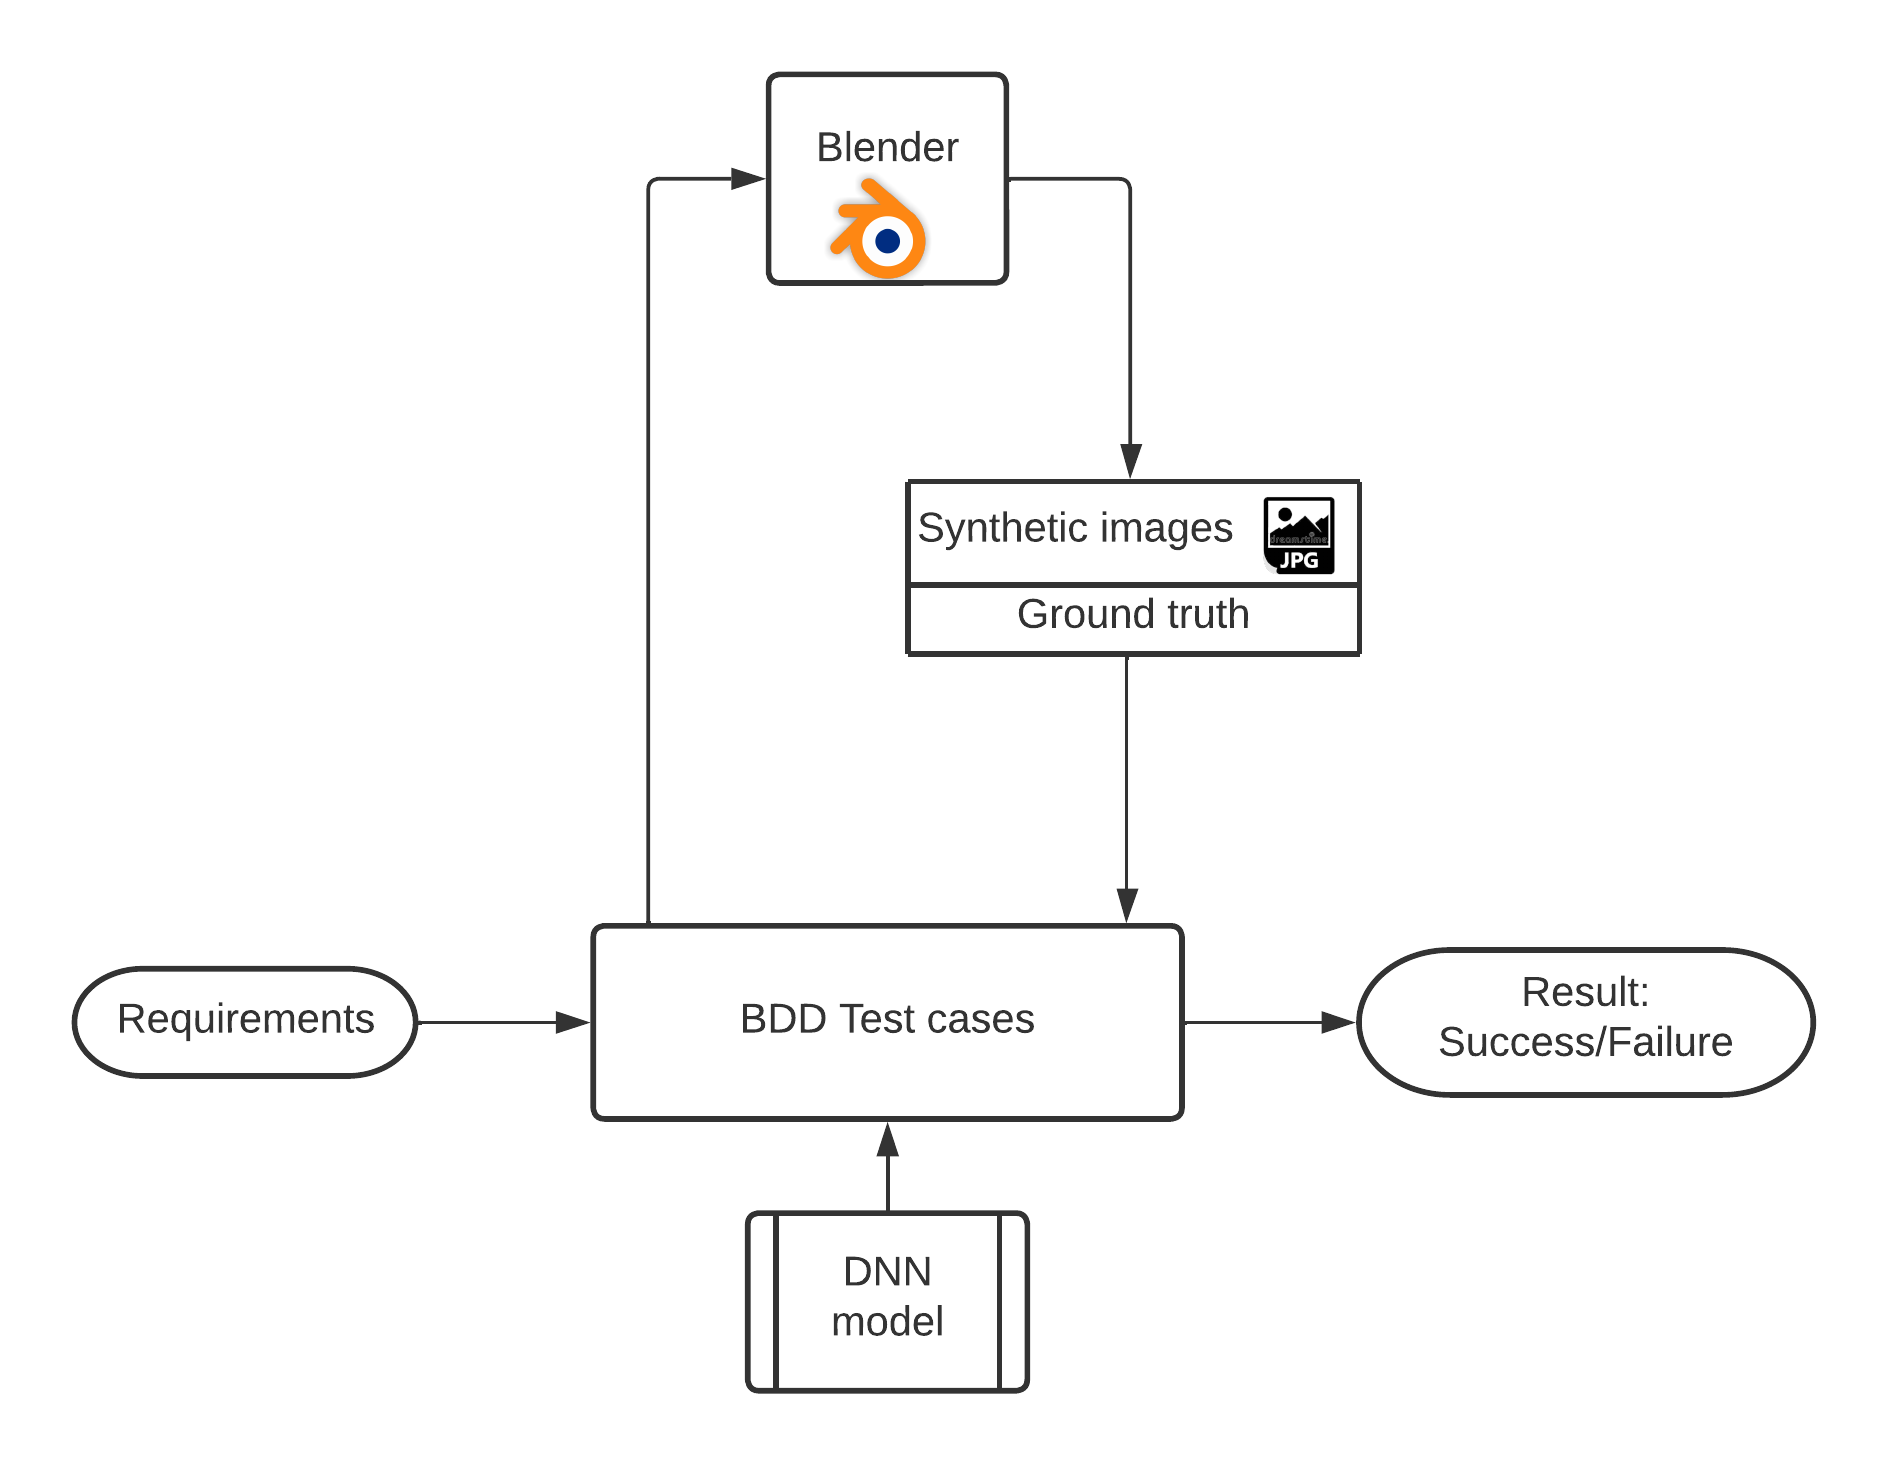
\includegraphics[scale=0.8]{images/basic block.png}
        \caption{The basic block diagram of the testing process}
        \label{fig:basic_block_diagram}
    \end{figure}
    
    \item Why is it essential to test a DNN?
    
    \begin{itemize}
        \item The most verified process of testing deep neural networks is to use test datasets. This aspect of testing is more viable and trusted than the other aspects of testing.
        \item In most DNN image classifiers, the trained models misunderstands one class with the other, or even sometimes show one-sided biases. Hence the properties of the class are violated and misinterpreted.
        \item Some DNNs perform well on simple tasks, but when it comes to the point to expand its use case, the user might begin to face capability issues from the model.
        \item We could never say a DNN model is perfectly trained and can perform well on any situation, because the possibilities real world inputs to this model is infinite.
    \end{itemize}
    
    \item An example of the testing process:
    
    One sample requirement from the test engineer could be
    
    \quad \textbf{Given} there is a DNN classifier model trained using a particular dataset,
    
    \quad \textbf{When} the model is tested using synthetic images with varying illuminance of 100-200 lux
    
    \quad \textbf{Then} the model must correctly classify the images
    
    During the when step of this requirement, the desired dataset along with its ground truth is generated and classified using the model, and in the then step the results are verified.
    
\end{itemize}

\subsection{Problem Statement}

Though Deep Neural Networks (DNNs) are being used extensively in many fields including safety critical systems such as autonomous driving and medical diagnostics, there are chances for the DNN to exhibit erroneous behaviours.

Unlike classical software testing, in AI testing after a model is trained, we have no clue whats happening inside all those networks, it just happens. Hence the best option is to follow the black-box testing approach in which we test the functionality of the software from the outside. During this process, this work aims to answer the following research questions.


    
\textbf{Research Questions:}

\begin{itemize}
    \begin{itemize}
        \item[\textbf{RQ1}] What are all the parameters that can be varied in blender for dataset generation?
        \item[\textbf{RQ2}] What are the requirements for testing a vision based DNN?
        \item[\textbf{RQ3}] What are the requirements from the test engineers for verifying DNNs?
        \item[\textbf{RQ4}] How to design a DSL for DNN testing based on requirements from test engineers and capabilities of blender?
        \item[\textbf{RQ5}] How DSL generated synthetic dataset benefits AI testing?
    \end{itemize}

\end{itemize}


\section{Related Work}
\begin{itemize}
    \item In this paper \cite{DBLP:journals/corr/abs-2112-12591}, the authors investigate black-box input diversity metrics as an alternative to white-box coverage criteria. They first select and adapt three diversity metrics and study, in a controlled manner, their capacity to measure actual diversity in input sets. Then they analyse their statistical association with fault detection using two datasets and three DNN models. They further compare diversity with state-of-the-art white-box coverage criteria. From the experiments, it could be inferred that relying on the diversity of image features embedded in test input sets is a more reliable indicator than coverage criteria to effectively guide the testing of DNNs. One of our selected black-box diversity metrics far outperforms existing coverage criteria in terms of fault-revealing capability and computational time. Results also confirm that state-of-the-art coverage metrics are not adequate to guide the construction of test input sets to detect as many faults as possible with natural inputs.
    
    \item In this paper \cite{DBLP:journals/corr/abs-1803-04792} , inspired by the MC/DC coverage criterion, the authors propose a family of four novel test criteria that are tailored to structural features of DNNs and their semantics. They validate the criteria by demonstrating that the generated test inputs guided via the proposed coverage criteria are able to capture undesired behaviours in a DNN. Test cases are generated using a symbolic approach and a gradient-based heuristic search. By comparing them with existing methods, they prove that their criteria achieve a balance between their ability to find bugs (proxied using adversarial examples) and the computational cost of test case generation. Experiments are conducted on state-of-the-art DNNs obtained using popular open source datasets, including MNIST, CIFAR-10 and ImageNet.
    
    \item In this paper \cite{10.1145/3180155.3180220}, the authors design, implement, and evaluate DeepTest, a systematic testing tool for automatically detecting erroneous behaviors of DNN-driven vehicles that can potentially lead to fatal crashes. A tool is designed to automatically generated test cases leveraging real-world changes in driving conditions like rain, fog, lighting conditions, etc. DeepTest systematically explore different parts of the DNN logic by generating test inputs that maximize the numbers of activated neurons. DeepTest found thousands of erroneous behaviors under different realistic driving conditions (e.g., blurring, rain, fog, etc.) many of which lead to potentially fatal crashes in three top performing DNNs in the Udacity self-driving car challenge.
    
    \item In this paper \cite{9780790}, the authors summarize some of the available tools for creating a synthetic dataset for object segmentation and provide a detailed example using the Blender 3D creation suite. They discuss in detail about the vital points and considerations for automatic dataset generation for object segmentation.
    
    \item There are many parallels between meta-modelling—in the sense of model-driven engineering—and meta-learning. Both rely on abstractions, the meta data, to model a predefined class of problems and to define the variabilities of the models conforming to this definition. Both are used to define the output and input relationships and then fitting the right models to represent that behaviour. In this paper \cite{8906948} , the authors envision how a meta-model for meta-learning can look like. THey discuss possible variabilities, for what types of learning it could be appropriate for, how concrete learning models can be generated from it, and how models can be finally selected. They also discuss a possible integration into existing modelling tools.
    
    \item This survey paper \cite{HUANG2020100270} conducts a review of the current research effort into making DNNs safe and trustworthy, by focusing on four aspects: verification, testing, adversarial attack and defence, and interpretability. In total, they survey 202 papers, most of which were published recently after 2017.
    
    \item In this paper \cite{9283925}, The authors propose a technique that re-purposes software testing methods, specifically mutation-based fuzzing, to augment the training data of DNNs, with the objective of enhancing their robustness. This technique casts the DNN data augmentation problem as an optimization problem. It uses genetic search to generate the most suitable variant of an input data to use for training the DNN, while simultaneously identifying opportunities to accelerate training by skipping augmentation in many instances. They instantiate this technique in two tools, Sensei and Sensei-SA, and evaluate them on 15 DNN models spanning 5 popular image data-sets. The evaluation shows that Sensei can improve the robust accuracy of the DNN, compared to the state of the art, on each of the 15 models, by upto 11.9\% and 5.5\% on average. Further, Sensei-SA reduces the average DNN training time by 25\%, while still improving robust accuracy.
    
\end{itemize}

\subsection{Subsection 1}
\subsection{Subsection 2}



\section{Project Plan}

\subsection{Work Packages}
The bare minimum will include the following packages:
\begin{enumerate}
    \item[WP1] Literature review on testing and verification of Deep Neural Networks
    \begin{itemize}
        \item[T1.1] Understanding verification and testing of Deep Neural Networks and the concept of synthetic dataset generation.
        \item[T1.2] Literature search on the testing and verification methods introduced in the past.
        \item[T1.3] Identify and analyse the state-of-the-art methods.
    \end{itemize}
    \item[WP2] Experimental setup
    \begin{itemize}
        \item[T2.1] Choose the best synthetic dataset generation tool and analyse its capabilities.
        \item[T2.2] Decide on the DNN models to be used for the verification.
        \item[T2.3] Gather requirements from a test engineer.
        \item[T2.4] Choose a suitable model to model transfer method to build a DSL that transfers requirements into dataset along with the ground truth.
    \end{itemize}
    \item[WP3] Mid-term Report
    \begin{itemize}
        \item[T3.1] Submission of the mid-term report.
    \end{itemize}
    \item[WP4] Experimental analysis
    \begin{itemize}
        \item[T4.1] Train the DNN model with the synthetic dataset.
        \item[T4.2] Follow a behaviour driven development method.
        \item[T4.3] The DSL creates dataset based on the requirements from the test engineer.
        \item[T4.4] The DNN model is tested using the created dataset.
        \item[T4.5] Verify the performance of the model.
    \end{itemize}
    \item[WP5] Final Report
    \begin{itemize}
        \item[T5.1] Draft revision.
        \item[T5.2] Submission of the Final report.
    \end{itemize}
    
\end{enumerate}

\subsection{Milestones}
\begin{enumerate}
    \item[M1] Literature search
    \item[M2] Experimental setup
    \item[M3] Mid-term Report submission
    \item[M4] Experimental Analysis
    \item[M5] Final Report submission
\end{enumerate}

\subsection{Project Schedule}
Include a gantt chart here. It doesn't have to be detailed, but it should include the milestones you mentioned above.
Make sure to include the writing of your report throughout the whole project, not just at the end.
    
\begin{figure}[h!]
    \centering
    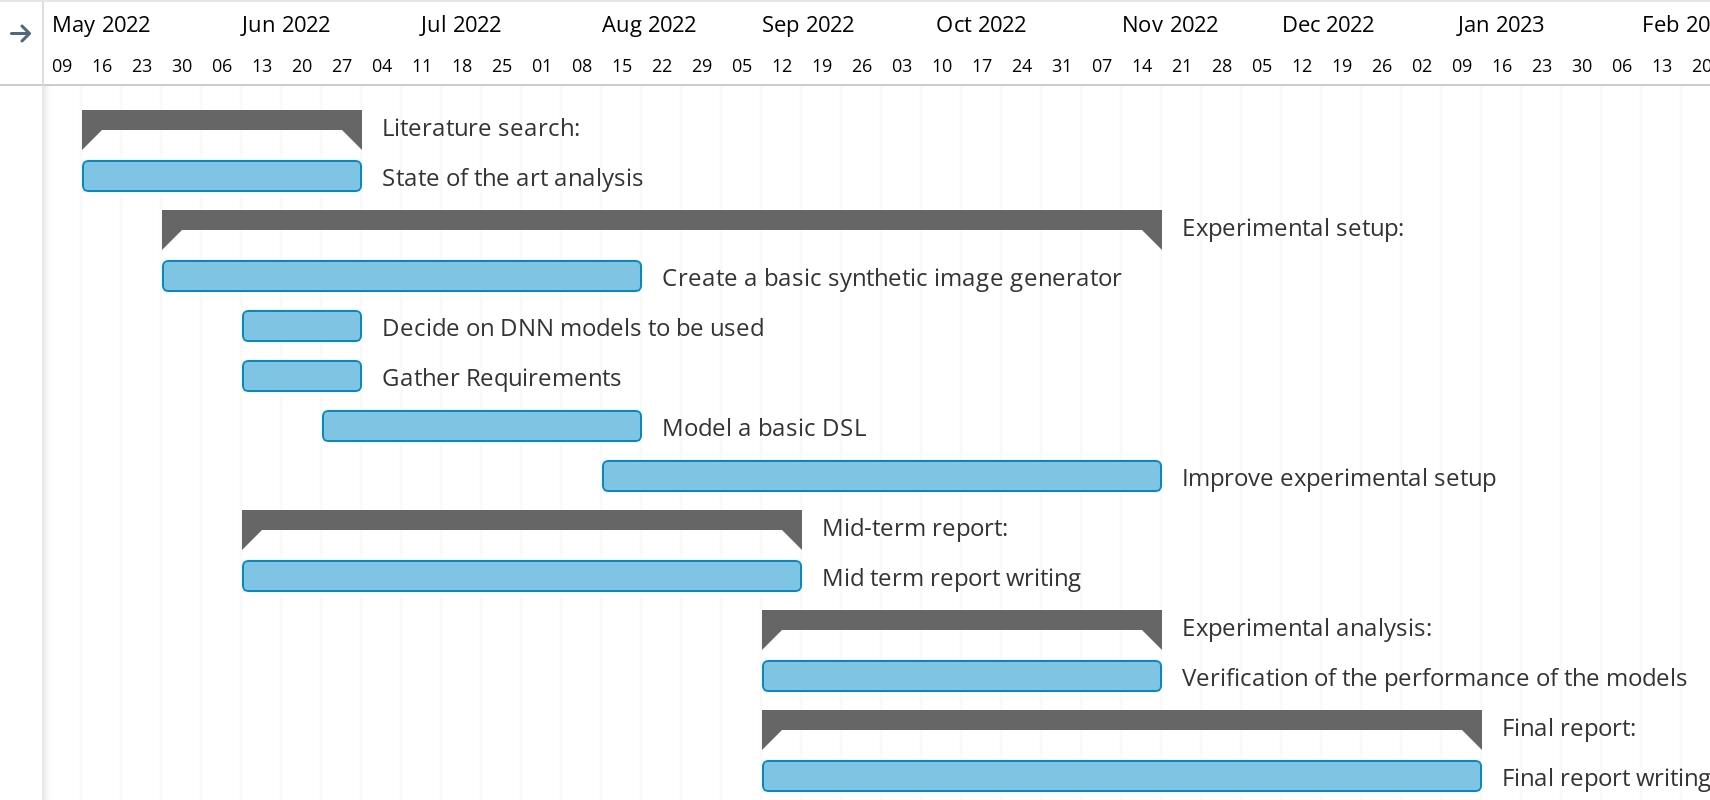
\includegraphics[width=\textwidth]{images/gantt.jpeg}
    \caption{The gantt chart of the RnD project}
    \label{fig:gantt_chart}
\end{figure}

\subsection{Deliverables}
\subsubsection*{Minimum Viable}

\begin{itemize}
    \item State of the art analysis.
    \item A simple and easy to use synthetic dataset generator with variabilies such as illumninance, sharpness, color, contrast, exposure, object poses, camera angles, FOV and perspective.
    \item Training the DNN with the synthetic data generated randomly irrespective of the requirements.
    \item A DSL that could map requirements to dataset generation functions and DNN testing functions.
    \item Verification of the DNN model for a classification or a regression application.
\end{itemize}

\subsubsection*{Expected}
\begin{itemize}
    \item A simple and easy to use synthetic dataset generator with additional variabilities such as material texture and reflection, crowded environment.
    \item Training the DNN with both synthetic and real world data on a ratio 3:1 respectively.
    \item Verification of the DNN model for a classification and a regression application.
\end{itemize}

\subsubsection*{Desired}
\begin{itemize}
    \item An easy to use synthetic dataset generator which could incorporate as much variabilities available in blender.
    \item Training the DNN with relatively more real world data than the synthetic data.
\end{itemize}


\nocite{*}

\bibliographystyle{plainnat} % Use the plainnat bibliography style
\bibliography{bibliography.bib} % Use the bibliography.bib file as the source of references




\end{document}
